\documentclass[11pt,letterpaper]{article}
\usepackage[T1]{fontenc}
\usepackage[utf8]{inputenc}
\usepackage{lmodern}
\usepackage[margin=0.95in]{geometry}
\usepackage{amsmath,amssymb,amsthm,mathtools}
\usepackage{microtype,graphicx,booktabs,enumitem}
\usepackage[font=small,labelfont=bf]{caption}
\usepackage{xcolor}
\definecolor{ink}{HTML}{173F4B}
\usepackage[colorlinks=true,linkcolor=ink,citecolor=ink,urlcolor=ink,breaklinks=true]{hyperref}
\usepackage[nameinlink,noabbrev]{cleveref}
\hypersetup{pdftitle={A sharp transition for conditioned spectral quantiles},pdfauthor={Research note prepared for Vladimir Reshetnikov}}
\setlength{\emergencystretch}{2em}
\setlength{\parskip}{0.25em}
\setlist{itemsep=0.25em,topsep=0.4em}
\numberwithin{equation}{section}
\newtheorem{theorem}{Theorem}[section]
\newtheorem{lemma}[theorem]{Lemma}
\newtheorem{proposition}[theorem]{Proposition}
\newtheorem{corollary}[theorem]{Corollary}
\theoremstyle{definition}
\newtheorem{definition}[theorem]{Definition}
\theoremstyle{remark}
\newtheorem{remark}[theorem]{Remark}
\newcommand{\PP}{\mathbb P}
\newcommand{\EE}{\mathbb E}
\newcommand{\QQ}{\mathbb Q}
\newcommand{\RR}{\mathbb R}
\newcommand{\dd}{\,\mathrm d}
\newcommand{\ind}{\mathbf 1}
\newcommand{\Var}{\operatorname{Var}}
\newcommand{\arctanh}{\operatorname{artanh}}
\newcommand{\Gam}{\operatorname{Gamma}}
\newcommand{\rate}{\mathcal R_\tau}
\newcommand{\mrate}{\mathcal R}
\newcommand{\starp}{c_*}
\newcommand{\commit}{\texttt{2e714ce3d8e33aa8160391cf5dd95f3af3c34045}}
\title{\vspace{-1em}\textbf{A sharp transition for conditioned spectral quantiles}\\[0.45em]
\large Exact rates, limiting profiles, and reciprocal $L$-function laws}
\author{Research note prepared for Vladimir Reshetnikov}
\date{27 November 2026}
\begin{document}
\maketitle
\begin{abstract}
Independent positive weights placed on a deterministic spectrum produce a random weighted sum. Conditioning this sum to be very small creates a predictable distribution of mass over the spectrum. We determine what happens when one also forces a fixed fraction of the mass above an unusually high spectral cutoff. There is an explicit transition: below it the sum remains close to the imposed upper bound; above it the typical sum becomes a strictly smaller fraction of that bound. For the median and a zeta-type spectrum, the transition occurs at $c_*=1.626121264897106\ldots$, and the large-deviation rate becomes exactly affine beyond it. We prove the result for every regularly varying counting function of index $\alpha$ and every inverse-power weight of exponent $p>\alpha$, identify the full conditional mass profile, and compute a strict jump in the second derivative of the rate. The probability theorem is unconditional. Its interpretation as a reciprocal completed $L$-function law uses the relevant Riemann hypothesis as an explicit input. The proof is self-contained apart from standard elementary probability and regular-variation estimates, and the accompanying code independently checks constants, identities, and finite discrete saddles.
\end{abstract}
\setcounter{tocdepth}{1}
\tableofcontents
\clearpage

\section{The result in a concrete form}\label{sec:concrete}

Let $0<\gamma_1\le\gamma_2\le\cdots$ be a deterministic list of positive numbers, with repetitions allowed, whose count grows like $T\log T$. Positive zero ordinates of the Riemann zeta function are the motivating example. Place independent exponential random variables $E_j$, each of mean one, on these numbers and form
\begin{equation}\label{eq:exampleX}
 X=\sum_{j\ge1}\frac{E_j}{\gamma_j^2}.
\end{equation}
The sum is almost surely finite. Its \emph{spectral median} is the height at which half its mass has accumulated:
\begin{equation}\label{eq:exampleH}
 H=\min\left\{\gamma_j:\sum_{\gamma_i\le\gamma_j}\frac{E_i}{\gamma_i^2}\ge\frac X2\right\}.
\end{equation}
For a small number $x>0$, define the exact scale $u=u(x)$ by
\begin{equation}\label{eq:examplesaddle}
 \sum_j\frac1{\gamma_j^2+u^2}=x.
\end{equation}
The existing conditional law in the source repository says that, given $X\le x$, the total is close to $x$, and the cumulative fraction below height $ru$ approaches $2\arctan(r)/\pi$ \cite{ProveIt}. Thus $H/u$ approaches one. We study the additional, exponentially unlikely event $H>cu$ for a fixed $c>1$.

\begin{theorem}[An explicit median transition]\label{thm:medianintro}
Suppose $N(T)=\#\{j:\gamma_j\le T\}$ is regularly varying of index one. Let $w\in(0,1)$ be the unique solution of
\begin{equation}\label{eq:wmedian}
 \arctan(1/w)=\arctanh w,
\end{equation}
and define
\begin{equation}\label{eq:medianconstants}
 c_* =\frac{4\arctanh w}{\pi w}
      =1.626121264897106\ldots,
 \qquad K=\log\frac{1+w^2}{1-w^2}
      =1.205197570560095\ldots.
\end{equation}
For every fixed $c>1$, conditioning on both $X\le x$ and $H>cu$ gives
\begin{equation}\label{eq:medianmass}
 \frac Xx\ \longrightarrow\ \min\{1,c_*/c\}
 \qquad\text{in probability as }x\downarrow0.
\end{equation}
Moreover
\begin{equation}\label{eq:medianLD}
 \log\PP(H>cu\mid X\le x)
 =-N(u)\,\mrate(c)+o(N(u)),
\end{equation}
where $\mrate(c)>0$ is given explicitly in \cref{sec:explicit}. For $c\ge c_*$,
\begin{equation}\label{eq:medianlinear}
 \boxed{\mrate(c)=Kc-\pi/2.}
\end{equation}
The rate is continuously differentiable at $c_*$, but its second derivative drops from $1.773642882285867\ldots$ on the left to zero on the right.
\end{theorem}

The conclusion concerns the mechanism of an unusually late median. For $1<c<c_*$, that event redistributes a total still close to $x$. For $c>c_*$, the most likely configuration also decreases the total. For example, imposing $H>2u$ makes $X/x$ approach $0.813060632448553\ldots$; imposing $H>3u$ makes it approach $0.542040421632369\ldots$. These are limits under the two conditioning events, not assertions about individual zero ordinates.

\begin{figure}[t]
 \centering
 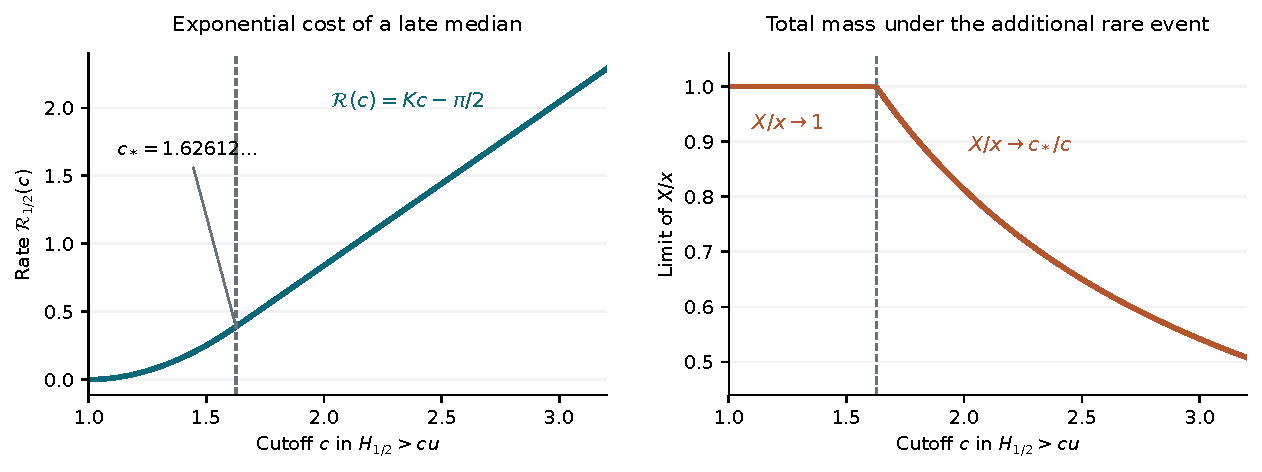
\includegraphics[width=\textwidth]{figures/phase_transition.pdf}
 \caption{The median transition for an index-one spectrum with inverse-square weights. The left panel shows the exact dimensionless rate. The right panel shows the limiting total after both conditioning events. The dotted line marks $c_*$.}
 \label{fig:transition}
\end{figure}

The exact equations in \cref{eq:wmedian,eq:medianconstants} define the constants; the displayed decimals are numerical evaluations. The theorem also holds with gamma weights of any fixed shape $\theta>0$. Then $N(u)$ in the exponential speed becomes $\theta N(u)$, while $c_*$ and $K$ remain unchanged.

\section{Source analysis, contribution, and prior work}\label{sec:source}

The inspected source is the GRH directory in Vladimir Reshetnikov's \emph{ProveIt} repository, pinned at revision \texttt{2e714ce3d8e3} (the full hash is recorded in \cite{ProveIt}). Its README describes an article assembled from 194 earlier research reports. The relevant chain of results is in \texttt{Article/sections/ana.tex}; the exact labels provide stable mathematical cross-references:
\begin{center}
\begin{tabular}{@{}p{0.36\textwidth}p{0.58\textwidth}@{}}
\toprule
Source label & Result used for comparison \\
\midrule
\texttt{ana:thm:gammasum} & Small-value asymptotics for weighted gamma sums. \\
\texttt{ana:thm:condlaw} & Typical conditional mass profile and finite-dimensional bridge limits. \\
\texttt{ana:thm:block} & Growing low-coordinate blocks and the sharp rate-correction threshold. \\
\texttt{ana:thm:macro} & Exact limiting loss of independence for macroscopic blocks. \\
\texttt{ana:thm:medianheight} & Gaussian fluctuations of the typical median, with a corrected center. \\
\bottomrule
\end{tabular}
\end{center}

The present contribution concerns a different scale. A fixed $c$ beyond the typical quantile imposes a deviation of order one in scaled height, whereas the earlier median theorem describes fluctuations tending to zero. We determine the exact large-deviation cost of that event, solve its constrained minimization, identify the additional transition at $c_*$, and prove the full limiting mass profile under the rare conditioning. These statements are not contained in the inspected source results. The new arguments are proved below; they do not require a functional central limit theorem.

Reciprocal-$\xi$ probability laws and the use of Hadamard products in Laplace transforms have established antecedents \cite{RoynetteYor,Gao}. The source also cites Sra's work on positivity properties of $\Xi$ and a tilted local limit calculation \cite{Sra}. Weighted gamma sums have also been studied directly in the large-deviation literature \cite{Saulis}. General maximum-entropy and Gibbs-conditioning principles, including weighted random measures, are classical \cite{VanCampenhoutCover,Gozlan}; conditional moments of small Gaussian ellipsoids were studied by Mayer-Wolf and Zeitouni \cite{MayerWolfZeitouni}. We do not claim those mechanisms as new. The proposed contribution is the explicit spectral-quantile rate, its transition, and its associated profile. A targeted literature search did not locate this exact theorem, which is a narrower statement than a certification of worldwide novelty.

\paragraph{Logical dependence.}
The general probability theorem assumes only the deterministic counting hypothesis stated below. It is therefore independent of RH and GRH. To identify its random sum with the reciprocal of a specified completed $L$-function, one additionally uses the corresponding critical-line zero statement and the paired Hadamard factorization. The source repository takes its stated RH/Dirichlet-GRH input as given. Sutherland's primary verification page reports successful builds of the shorter Lean development and axiom audits containing \texttt{propext}, \texttt{Classical.choice}, and \texttt{Quot.sound} \cite{Sutherland}. This note records the input and that external verification report; it does not independently rerun the upstream development. No Lean formalization of the new theorem is claimed.

\section{The general theorem}\label{sec:general}

\subsection{Spectrum, scale, and quantile}

Fix $\alpha>0$, $p>\alpha$, and $\theta>0$. Let
\begin{equation}\label{eq:RV}
 0<\gamma_1\le\gamma_2\le\cdots\longrightarrow\infty,
 \qquad N(T)=\#\{j:\gamma_j\le T\},
 \qquad \frac{N(rT)}{N(T)}\longrightarrow r^\alpha\quad(r>0).
\end{equation}
Let $G_j$ be independent $\Gam(\theta,1)$ variables, where the second parameter is the rate, and put
\begin{equation}\label{eq:Xgeneral}
 X=\sum_j\frac{G_j}{\gamma_j^p}.
\end{equation}
For $0<x<\EE X$, choose the unique positive $t=u^p$ satisfying
\begin{equation}\label{eq:exact_saddle}
 \theta\sum_j\frac1{\gamma_j^p+t}=x,
 \qquad n=N(u).
\end{equation}
Existence, uniqueness, and finiteness of the sum are proved in \cref{sec:sums}. Define
\begin{equation}\label{eq:CD}
 \nu(\dd r)=\alpha r^{\alpha-1}\dd r,
 \qquad C=\int_0^\infty\frac{\nu(\dd r)}{1+r^p}
       =\frac{\alpha\pi}{p\sin(\pi\alpha/p)},
 \qquad D=\left(\frac p\alpha-1\right)C.
\end{equation}
In particular $C,D>0$. The exact saddle gives $tx/(\theta n)\to C$.

For a fixed fraction $\tau\in(0,1)$, define
\begin{equation}\label{eq:Htau}
 H_\tau=\min\left\{\gamma_j:
 \sum_{\gamma_i\le\gamma_j}\frac{G_i}{\gamma_i^p}\ge\tau X\right\}.
\end{equation}
All coordinates with the same ordinate are included together. The typical cutoff $c_0>0$ is the unique solution of
\begin{equation}\label{eq:c0}
 \int_0^{c_0}\frac{\nu(\dd r)}{1+r^p}=\tau C.
\end{equation}
For $c>0$, write
\begin{equation}\label{eq:LR}
 L_c(a)=\int_0^c\frac{\nu(\dd r)}{r^p+a}\quad(a>0),
 \qquad R_c(b)=\int_c^\infty\frac{\nu(\dd r)}{r^p+b}\quad(b>-c^p).
\end{equation}
Each is a smooth strictly decreasing bijection, from its indicated parameter interval onto $(0,\infty)$.

\subsection{The transition constants}

Set $k=\tau/(1-\tau)$. There is a unique $A\in(0,1/k)$ such that, with $B=-kA$,
\begin{equation}\label{eq:AB}
 \frac{L_1(A)}{R_1(B)}=k.
\end{equation}
Indeed, as $A$ increases, the numerator decreases from infinity and the denominator increases to infinity. Define
\begin{equation}\label{eq:cstar}
 M=L_1(A)+R_1(B),\qquad
 c_*=(M/C)^{1/(p-\alpha)},\qquad
 K=\log\frac{1+A}{1+B}.
\end{equation}
We will prove $c_*>c_0$; also $K>0$ because $A>0>B>-1$.

\begin{theorem}[Exact rate and total-mass transition]\label{thm:main}
Under \cref{eq:RV}, fix $\tau\in(0,1)$ and $c>c_0$. Then
\begin{equation}\label{eq:rate_limit}
 \lim_{x\downarrow0}\frac1{\theta N(u)}
 \log\PP(H_\tau>cu\mid X\le x)=-\rate(c).
\end{equation}
The rate is given by the following two formulas.
\begin{enumerate}[label=\textup{(\roman*)}]
\item If $c_0<c<c_*$, let $a>0$ and $b>-c^p$ be the unique solutions
\begin{equation}\label{eq:boundary_rates}
 L_c(a)=\tau C,\qquad R_c(b)=(1-\tau)C,
 \qquad \lambda=\tau a+(1-\tau)b.
\end{equation}
Then $a>b$, $\lambda>0$, and
\begin{equation}\label{eq:boundary_rate}
 \boxed{\rate(c)=c^\alpha\log\frac{c^p+a}{c^p+b}+D(\lambda-1).}
\end{equation}
\item If $c\ge c_*$, use $a=c^pA$ and $b=c^pB$, so that $\lambda=0$. Then
\begin{equation}\label{eq:interior_rate}
 \boxed{\rate(c)=c^\alpha K-D.}
\end{equation}
\end{enumerate}
The formulas agree at $c_*$. The rate is positive and strictly increasing on $(c_0,\infty)$ and tends to zero as $c\downarrow c_0$.

Conditionally on both $X\le x$ and $H_\tau>cu$,
\begin{equation}\label{eq:general_total}
 \boxed{\frac Xx\longrightarrow
 \min\left\{1,\left(\frac{c_*}{c}\right)^{p-\alpha}\right\}}
\end{equation}
in probability. Moreover
\begin{equation}\label{eq:fraction_limit}
 \frac1X\sum_{\gamma_j\le cu}\frac{G_j}{\gamma_j^p}\longrightarrow\tau
 \qquad\text{in probability under the same conditioning.}
\end{equation}
\end{theorem}

Negative $b$ is allowed only on the upper band $r>c$, where $r^p+b>0$. It does not represent a negative gamma rate. At $c=c_*$ the total in \cref{eq:general_total} still tends to $x$; a positive macroscopic gap below $x$ appears only beyond the transition.

\begin{theorem}[Complete conditional mass profile]\label{thm:profile}
Use the rates $a,b$ prescribed by \cref{thm:main}, and define, for $r\in[0,\infty]$,
\begin{equation}\label{eq:profile}
 F_c(r)=\frac1C\left\{
 \int_0^{\min(r,c)}\frac{\nu(\dd v)}{v^p+a}
 +\ind_{\{r>c\}}\int_c^r\frac{\nu(\dd v)}{v^p+b}\right\}.
\end{equation}
Conditionally on $X\le x$ and $H_\tau>cu$,
\begin{equation}\label{eq:uniform_profile}
 \sup_{0\le r\le\infty}
 \left|\frac1x\sum_{\gamma_j\le ru}\frac{G_j}{\gamma_j^p}-F_c(r)\right|
 \longrightarrow0
 \qquad\text{in probability.}
\end{equation}
In particular $F_c(\infty)$ equals the total-mass limit in \cref{eq:general_total}. Dividing $F_c$ by $F_c(\infty)$ gives the limiting profile normalized by the actual total $X$.
\end{theorem}

\begin{theorem}[A strict change in the curvature]\label{thm:curvature}
The function $\rate$ is smooth on each side of $c_*$ and continuously differentiable at $c_*$. Put $a_*=c_*^p A$, $b_*=c_*^p B$, and
\begin{equation}\label{eq:UV}
 U=\int_0^{c_*}\frac{\nu(\dd r)}{(r^p+a_*)^2},\qquad
 V=\int_{c_*}^\infty\frac{\nu(\dd r)}{(r^p+b_*)^2}.
\end{equation}
Then
\begin{equation}\label{eq:jump}
 \boxed{\rate''(c_*-)-\rate''(c_*+)
 =\frac{(p-\alpha)^2C^2}{c_*^2}
 \left(\frac{\tau^2}{U}+\frac{(1-\tau)^2}{V}\right)>0.}
\end{equation}
The right-hand second derivative is $\alpha(\alpha-1)c_*^{\alpha-2}K$. In particular it is zero when $\alpha=1$.
\end{theorem}

\section{Spectral sums and the exact saddle}\label{sec:sums}

\begin{lemma}[Spectral summation]\label{lem:sums}
The measures $\nu_u=N(u)^{-1}\sum_j\delta_{\gamma_j/u}$ converge vaguely on $(0,\infty)$ to $\nu$. Suppose $f$ is locally bounded on $(0,\infty)$, is bounded near zero, is continuous apart from finitely many fixed positive points, and satisfies $f(r)=O(r^{-p})$ at infinity. Then
\begin{equation}\label{eq:sum_limit}
 \frac1{N(u)}\sum_j f(\gamma_j/u)
 \longrightarrow\int_0^\infty f(r)\nu(\dd r).
\end{equation}
The same holds after restricting the sum and integral to either side of a fixed positive cutoff. Also $\sum_j\gamma_j^{-p}<\infty$.
\end{lemma}

\begin{proof}
For $0<a<b<\infty$, regular variation gives
\[
 \nu_u((a,b])=\frac{N(bu)-N(au)}{N(u)}\longrightarrow b^\alpha-a^\alpha.
\]
This proves convergence on compact intervals away from zero. The limiting measure has no atoms at the finitely many discontinuities. Below $\delta$, boundedness of $f$ bounds the limiting upper contribution by a constant times $\delta^\alpha$.

For the tail, choose $\varepsilon\in(0,p-\alpha)$. The standard dyadic bound from regular variation gives, for $u$ sufficiently large and $r\ge1$,
\[
 \frac{N(ru)}{N(u)}\le C_\varepsilon r^{\alpha+\varepsilon}.
\]
One can obtain this directly by first making $N(2T)/N(T)\le2^{\alpha+\varepsilon}$ for all sufficiently large $T$ and then iterating, with one extra factor to cover intermediate $r$. Consequently
\[
 \frac1{N(u)}\sum_{\gamma_j/u>R}(\gamma_j/u)^{-p}
 \le C\sum_{m\ge0}(2^mR)^{-p}(2^{m+1}R)^{\alpha+\varepsilon},
\]
which tends to zero uniformly in large $u$ as $R\to\infty$. Truncation now proves \cref{eq:sum_limit}. The same dyadic argument at a fixed sufficiently large starting height proves the convergence of $\sum_j\gamma_j^{-p}$.
\end{proof}

It follows that $\EE X=\theta\sum_j\gamma_j^{-p}<\infty$, so $X<\infty$ almost surely. The left side of \cref{eq:exact_saddle} is continuous and strictly decreasing in $t\ge0$, starts at $\EE X$, and tends to zero. Thus the exact saddle exists uniquely and $t,u\to\infty$ as $x\downarrow0$. By \cref{lem:sums},
\begin{equation}\label{eq:mu_limit}
 \mu_u:=\frac{tx}{\theta n}
 =\frac1{N(u)}\sum_j\frac1{1+(\gamma_j/u)^p}
 \longrightarrow C.
\end{equation}
The beta integral evaluates $C$ as in \cref{eq:CD}.

The event $X\le x$ has positive probability for every $x>0$. Indeed, choose a finite initial segment so that the remaining expected tail is below $x/4$. Markov's inequality gives positive probability that the tail is at most $x/2$, and independently the finitely many initial gamma variables can all be small enough to contribute at most $x/2$.

\section{A two-band large-deviation principle}\label{sec:LDP}

We give the probability argument explicitly. This both fixes the normalization and avoids any need for a large-deviation theorem on an infinite-dimensional space.

\subsection{The first exponential change of measure}

Let
\begin{equation}\label{eq:Laplace}
 \mathcal K(t)=\theta\sum_j\log(1+t/\gamma_j^p),
 \qquad \EE e^{-tX}=e^{-\mathcal K(t)},
 \qquad \frac{\dd\PP_t}{\dd\PP}=e^{-tX+\mathcal K(t)}.
\end{equation}
Fix $c>0$, split $X=X_1+X_2$ at $\gamma_j=cu$, and set
\begin{equation}\label{eq:Z}
 S_i=tX_i,\qquad Z_i=\frac{S_i}{\theta n}\quad(i=1,2).
\end{equation}
Under $\PP_t$, the variables $Y_j=tG_j/\gamma_j^p$ are independent gamma variables of shape $\theta$ and rate $1+(\gamma_j/u)^p$. The logarithm of the moment generating function, normalized by $\theta n$, converges to
\begin{align}\label{eq:Lambda}
 \Lambda_c(\lambda_1,\lambda_2)
 &=-\int_0^c\log\left(1-\frac{\lambda_1}{1+r^p}\right)\nu(\dd r)\notag\\
 &\quad-\int_c^\infty\log\left(1-\frac{\lambda_2}{1+r^p}\right)\nu(\dd r),
 \qquad \lambda_1<1,\quad\lambda_2<1+c^p.
\end{align}
For these fixed parameters, \cref{lem:sums} applies: the integrands are bounded near zero and decay as $O(r^{-p})$ at infinity. We denote the finite-$u$ normalized logarithm by $\Lambda_{c,u}$.

Write $\Lambda_c=\Lambda_{1,c}+\Lambda_{2,c}$. Each summand is smooth and strictly convex on its domain, with derivatives
\begin{equation}\label{eq:Lambda_derivative}
 \Lambda'_{1,c}(\lambda)=L_c(1-\lambda),\qquad
 \Lambda'_{2,c}(\lambda)=R_c(1-\lambda).
\end{equation}
Each derivative maps its domain bijectively onto $(0,\infty)$. At the upper endpoint, the first diverges because $p>\alpha$, and the second has a logarithmic divergence at $r=c$. At the lower endpoint $\lambda\to-\infty$, both tend to zero by dominated convergence. The second derivatives are finite and positive at every interior parameter.

\begin{lemma}[The tilted two-band law]\label{lem:tiltedLDP}
Under $\PP_t$, the vector $Z=(Z_1,Z_2)$ obeys a good large-deviation principle at speed $\theta n$, with rate
\begin{equation}\label{eq:I}
 I_c(z)=I_{1,c}(z_1)+I_{2,c}(z_2)=\Lambda_c^*(z).
\end{equation}
For $z_1,z_2>0$, there is a unique interior $\lambda$ with $\nabla\Lambda_c(\lambda)=z$, and
\begin{equation}\label{eq:I_eval}
 I_c(z)=\lambda\cdot z-\Lambda_c(\lambda).
\end{equation}
The rate is smooth and strictly convex on the positive quadrant and is infinite on either coordinate axis and outside the nonnegative quadrant.
\end{lemma}

\begin{proof}
For completeness, the upper bound follows from the Chernoff inequality. For any fixed interior parameter $\lambda$ and small neighborhood $B$ of a point $z$,
\[
 \PP_t(Z\in B)\le
 \exp\left\{\theta n\left(\Lambda_{c,u}(\lambda)
 -\inf_{y\in B}\lambda\cdot y\right)\right\}.
\]
Choose parameters approaching the Legendre supremum, cover a compact set by finitely many such neighborhoods, and pass to the limit. A fixed small positive parameter in both coordinates proves exponential tightness, completing the upper bound for closed sets.

For the lower bound at $z_1,z_2>0$, choose the unique parameter satisfying $\nabla\Lambda_c(\lambda)=z$ and further change measure by
\begin{equation}\label{eq:secondtilt}
 \frac{\dd\QQ_{u,\lambda}}{\dd\PP_t}
 =\exp\{\lambda_1S_1+\lambda_2S_2-\theta n\Lambda_{c,u}(\lambda)\}.
\end{equation}
The gamma rates become $1+r_j^p-\lambda_i$ on the two bands, where $r_j=\gamma_j/u$. The spectral lemma gives means of $Z$ tending to $z$. Its variances are $O(1/n)$, since the corresponding squared reciprocal rates have finite limiting integrals. Hence $\QQ_{u,\lambda}$ assigns probability tending to one to every fixed neighborhood of $z$. Bounding the inverse likelihood ratio on such a neighborhood gives the lower bound with exponent \cref{eq:I_eval}.

The derivative ranges proved above show that this treats every point in the positive quadrant. The rate on an axis is infinite: for example, $I_{1,c}(0)=\sup_\lambda[-\Lambda_{1,c}(\lambda)]=\infty$ because $\Lambda_{1,c}(\lambda)\to-\infty$ as $\lambda\to-\infty$. For the tail, restrict the integral to any fixed positive-length interval inside $(c,\infty)$ to obtain the same conclusion. Negative coordinates are impossible. Strict convexity and smoothness follow from the strictly positive second derivatives of the cumulants. Exponential tightness and the closed-set upper bound give a good rate function.
\end{proof}

\subsection{The exact moving conditioning boundary}

The event $X\le x$ corresponds to $Z_1+Z_2\le\mu_u$, where the boundary $\mu_u$ is defined by the exact saddle, not merely its leading approximation. Put
\begin{equation}\label{eq:D_u}
 D_u=\EE_t[e^{tX-tx}\ind_{\{X\le x\}}].
\end{equation}
Then $0<D_u\le1$ and
\begin{equation}\label{eq:D_subexp}
 \lim_{u\to\infty}\frac{\log D_u}{\theta n}=0.
\end{equation}
To prove the lower bound, let $z^0=\nabla\Lambda_c(0)$, whose coordinates sum to $C$. For fixed $\delta>0$, a sufficiently small neighborhood of $(1-\delta)z^0$ lies below $Z_1+Z_2\le\mu_u$ eventually. The lower bound from \cref{lem:tiltedLDP} gives, after shrinking that neighborhood,
\[
 \liminf\frac{\log D_u}{\theta n}
 \ge-\delta C-I_c((1-\delta)z^0).
\]
Letting $\delta\downarrow0$ proves \cref{eq:D_subexp}, since $I_c(z^0)=0$ and $I_c$ is continuous there. A local central limit theorem is unnecessary for this exponential normalization.

\begin{lemma}[The conditional two-band law]\label{lem:conditionalLDP}
Under $\PP(\,\cdot\mid X\le x)$, the vector $Z$ obeys a good large-deviation principle at speed $\theta n$, with rate
\begin{equation}\label{eq:J}
 J_c(z)=\begin{cases}
 I_c(z)-z_1-z_2+C,&z_1,z_2>0,\ z_1+z_2\le C,\\
 +\infty,&\text{otherwise}.
 \end{cases}
\end{equation}
Its minimum is zero at $z^0=\nabla\Lambda_c(0)$.
\end{lemma}

\begin{proof}
The exact density relative to $\PP_t$ is
\begin{equation}\label{eq:conditionalRN}
 \frac{\dd\PP(\,\cdot\mid X\le x)}{\dd\PP_t}
 =D_u^{-1}e^{\theta n(Z_1+Z_2-\mu_u)}
 \ind_{\{Z_1+Z_2\le\mu_u\}}.
\end{equation}
On the compact triangle $z_1+z_2\le C+\varepsilon$, a finite-cover argument applied to the continuous exponent $z_1+z_2$ and \cref{lem:tiltedLDP} yields the upper bound. Let $\varepsilon\downarrow0$ and use \cref{eq:D_subexp,eq:mu_limit}. This proves the closed-set upper bound with \cref{eq:J}; the conditioned measures have compact support in that enlarged triangle for large $u$.

For a positive point with $z_1+z_2<C$, a small neighborhood lies under the exact boundary for all large $u$, and \cref{eq:conditionalRN} transfers the open-set lower bound directly. A finite-rate point with $z_1+z_2=C$ is approximated from below by $(1-\delta)z$, which remains in any prescribed open neighborhood for small $\delta$. Continuity of $I_c$ on the positive quadrant then gives the same lower bound at the boundary. Axes have infinite rate and need no further lower bound. This establishes the claim without any assumption on the error $\mu_u-C$ beyond convergence to zero.
\end{proof}

\section{Solving the quantile constraint}\label{sec:optimization}

\subsection{Reduction to one scalar}

The event $H_\tau>cu$ is $X_1<\tau(X_1+X_2)$. Equality has probability zero: the two bands are independent, and each has a continuous distribution once the lower band is nonempty, as it is for all sufficiently large $u$. Thus its conditional exponential rate is the minimum of $J_c$ on
\begin{equation}\label{eq:feasible}
 \mathcal E_c=\{z_1,z_2\ge0:\ z_1\le\tau(z_1+z_2),\ z_1+z_2\le C\}.
\end{equation}
The infima over the closed event and its strict interior agree. Indeed, a finite-rate minimizer is positive and can be perturbed toward a positive point satisfying both inequalities strictly; continuity of $J_c$ then applies. Consequently the LDP gives the exact limit, rather than only upper and lower bounds.

The minimum exists and is unique: $\mathcal E_c$ is compact and convex, $J_c$ is lower semicontinuous and finite at a positive feasible point, infinite on the axes, and strictly convex wherever finite. At a positive point, write
\begin{equation}\label{eq:dualab}
 a=1-\partial_1 I_c(z)>0,\qquad
 b=1-\partial_2 I_c(z)>-c^p.
\end{equation}
Then
\begin{equation}\label{eq:meanab}
 z_1=L_c(a),\quad z_2=R_c(b),\quad\nabla J_c(z)=(-a,-b).
\end{equation}

For $c>c_0$, the quantile inequality is active at the minimizer. If both constraints were strict, increasing $z_1$ slightly would decrease $J_c$, because its first derivative is $-a<0$. If only the total constraint were active, stationarity along $z_1+z_2=C$ would force $a=b$. Scaling the full integral would then give
\[
 C=L_c(a)+R_c(a)=Ca^{\alpha/p-1},
\]
so $a=b=1$. But this point has lower-band fraction
\[
 C^{-1}\int_0^c\frac{\nu(\dd r)}{1+r^p}>\tau,
\]
contradicting feasibility. Hence the minimizer has the form
\begin{equation}\label{eq:line}
 z=(\tau s,(1-\tau)s),\qquad 0<s\le C.
\end{equation}

Set
\begin{equation}\label{eq:h}
 h(c,s)=I_{1,c}(\tau s)+I_{2,c}((1-\tau)s)-s+C.
\end{equation}
At the associated rates $a,b$,
\begin{align}\label{eq:h_derivs}
 h_s(c,s)&=-[\tau a+(1-\tau)b],\notag\\
 h_{ss}(c,s)&=\frac{\tau^2}{U_c(a)}+
 \frac{(1-\tau)^2}{V_c(b)}>0,
\end{align}
where
\[
 U_c(a)=\int_0^c\frac{\nu(\dd r)}{(r^p+a)^2},\qquad
 V_c(b)=\int_c^\infty\frac{\nu(\dd r)}{(r^p+b)^2}.
\]
As $s\downarrow0$, both $a,b$ tend to infinity and $h_s<0$ eventually. As $s\to\infty$, $a\to0$, $b\to-c^p$, and $h_s\to(1-\tau)c^p>0$. Therefore there is one unconstrained minimizer.

Its equation is $\tau a+(1-\tau)b=0$. Writing $a=c^pA$, $b=c^pB$ produces exactly \cref{eq:AB}. Scaling the integrals in \cref{eq:LR} gives the unconstrained total
\begin{equation}\label{eq:s0}
 s_0(c)=c^{\alpha-p}M=C(c_*/c)^{p-\alpha}.
\end{equation}
The constrained solution is consequently
\begin{equation}\label{eq:sbar}
 \boxed{\overline s(c)=\min\{C,s_0(c)\}.}
\end{equation}
At $c=c_0$, the boundary point has $a=b=1$ and $h_s(c_0,C)=-1<0$. Its unconstrained minimizer therefore lies beyond $C$, proving $c_*>c_0$. Below the transition $h_s(c,C)<0$, so $\lambda=\tau a+(1-\tau)b>0$. At fixed $s=C$, differentiating the two mean constraints shows that $a$ increases and $b$ decreases with $c$. Since they both equal one at $c_0$, we have $a>b$ above $c_0$. In the interior phase this is immediate from $A>0>B$.

\subsection{An exact integration identity}

Define
\begin{equation}\label{eq:F}
 \mathcal F_c(a,b)=\int_0^c\log\frac{r^p+a}{r^p+1}\nu(\dd r)
 +\int_c^\infty\log\frac{r^p+b}{r^p+1}\nu(\dd r).
\end{equation}
Integration by parts gives
\begin{equation}\label{eq:IBP}
 \mathcal F_c(a,b)=c^\alpha\log\frac{c^p+a}{c^p+b}
 +\frac p\alpha\{aL_c(a)+bR_c(b)-C\}.
\end{equation}
One direct derivation applies integration by parts separately to $\log(1+a/r^p)$ on $(0,c)$ and $\log(1+b/r^p)$ on $(c,\infty)$, and subtracts the corresponding full integral for parameter one. At zero, $r^\alpha\log r\to0$; at infinity the relevant logarithmic difference is $O(r^{-p})$, so all endpoint terms are valid. In particular
\[
 \int_0^\infty\log(1+r^{-p})\nu(\dd r)=\frac p\alpha C.
\]

Since $\Lambda_c(1-a,1-b)=-\mathcal F_c(a,b)$, Legendre duality gives
\begin{align}\label{eq:J_eval}
 J_c(L_c(a),R_c(b))
 &=\mathcal F_c(a,b)+C-aL_c(a)-bR_c(b)\notag\\
 &=c^\alpha\log\frac{c^p+a}{c^p+b}
 +\left(\frac p\alpha-1\right)
 \{aL_c(a)+bR_c(b)-C\}.
\end{align}
At the boundary solution, $aL+bR=\lambda C$; at the interior solution it is zero. This proves \cref{eq:boundary_rate,eq:interior_rate} and the probability limit in \cref{eq:rate_limit}.

The envelope derivative is
\begin{equation}\label{eq:rate_derivative}
 \rate'(c)=\alpha c^{\alpha-1}\log\frac{c^p+a}{c^p+b}>0
 \qquad(c>c_0),
\end{equation}
with the appropriate minimizing rates. For example, at fixed $s$ it follows by differentiating the two cumulant integrals at their common band endpoint; dependence of the optimizing dual parameters cancels by stationarity. In the interior phase it also follows directly from \cref{eq:interior_rate}. At $c=c_0$, $a=b=1$ and the rate is zero. Hence the rate is positive and strictly increasing thereafter.

\subsection{Concentration at the minimizing configuration}

The good conditional LDP and uniqueness imply concentration at the minimizer under the additional rare event. On the closed feasible set outside any fixed neighborhood of that point, the minimum rate exceeds $\rate(c)$ by a positive amount. Divide its exponential upper bound by the exact probability $\exp\{-\theta n\rate(c)+o(n)\}$ of the rare event. The resulting conditional probability tends to zero exponentially.

Therefore $Z_1+Z_2\to\overline s(c)$ and $Z_1/(Z_1+Z_2)\to\tau$. Since $X/x=(Z_1+Z_2)/\mu_u$ and $\mu_u\to C$, \cref{eq:sbar} proves \cref{eq:general_total,eq:fraction_limit}, completing \cref{thm:main}.

\section{Proof of the full conditional profile}\label{sec:profileproof}

Fix the minimizing rates $a,b$ from \cref{thm:main}. In \cref{eq:secondtilt}, take parameters $(1-a,1-b)$ and denote the resulting law by $\QQ_u$. Under it the variables $Y_j=tG_j/\gamma_j^p$ are independent gamma variables with rates
\begin{equation}\label{eq:profile_rates}
 r_j^p+a\quad(r_j\le c),\qquad
 r_j^p+b\quad(r_j>c).
\end{equation}
These rates are uniformly separated from zero on their respective bands: $a>0$ and $c^p+b>0$. Thus the moment generating functions used below are finite in a fixed neighborhood of zero.

On the event $X\le x$, $H_\tau>cu$, we have
\begin{align}\label{eq:key_bound}
 aS_1+bS_2
 &=\lambda(S_1+S_2)
 +(a-b)\{S_1-\tau(S_1+S_2)\}\notag\\
 &\le\lambda tx,
\end{align}
where $\lambda=\tau a+(1-\tau)b\ge0$ and $a>b$. Combining the two exact changes of measure gives
\begin{align}\label{eq:profileRN}
 \frac{\dd\PP(\,\cdot\mid X\le x)}{\dd\QQ_u}
 =D_u^{-1}\exp\{aS_1+bS_2-tx
 +\theta n\Lambda_{c,u}(1-a,1-b)\}
 \ind_{\{X\le x\}}.
\end{align}
Consequently, on the rare event, this density is bounded above by
\begin{equation}\label{eq:RN_bound}
 \exp\{-\theta n\rate(c)+o(n)\}.
\end{equation}
To see the exponent exactly, use
\[
 \rate(c)=C(1-\lambda)-\Lambda_c(1-a,1-b)
\]
in the boundary phase. In the interior phase $\lambda=0$, and the same equation holds. These identities also follow directly from \cref{eq:I_eval,eq:J} and the minimizing constraints.

Under $\QQ_u$, \cref{lem:sums} identifies the mean of each partial sum divided by $\theta n$ with the integrals defining $CF_c(r)$. For every fixed $r$ and $\varepsilon>0$, Chernoff's inequality gives
\begin{equation}\label{eq:profile_chernoff}
 \QQ_u\left(\left|
 \frac1{\theta n}\sum_{\gamma_j\le ru}Y_j-CF_c(r)
 \right|>\varepsilon\right)\le e^{-\delta n}
\end{equation}
for a suitable $\delta>0$ and all sufficiently large $u$. The proof is elementary: the normalized log moment generating function converges in a neighborhood of zero, its derivative at zero is the stated mean, and a sufficiently small positive or negative parameter gives a strictly negative Chernoff exponent. The same argument treats the full sum $r=\infty$.

Transfer \cref{eq:profile_chernoff} through \cref{eq:RN_bound} and divide by the rare-event probability from \cref{eq:rate_limit}. The factors $\exp\{-\theta n\rate(c)+o(n)\}$ cancel, leaving exponential decay. Therefore each fixed partial sum converges under the two conditioning events to $CF_c(r)$ on the $\theta n/t$ scale. The limit in \cref{eq:mu_limit} converts this to the $x$ scale.

Finally, $F_c$ is continuous and increasing on the compactified interval $[0,\infty]$. Choose a finite grid, including zero and infinity, on which successive values of $F_c$ differ by less than a prescribed tolerance. Monotonicity of the random partial sums and a union bound over the grid give uniform convergence. This proves \cref{thm:profile} without asserting an infinite-dimensional large-deviation principle.

\begin{figure}[t]
 \centering
 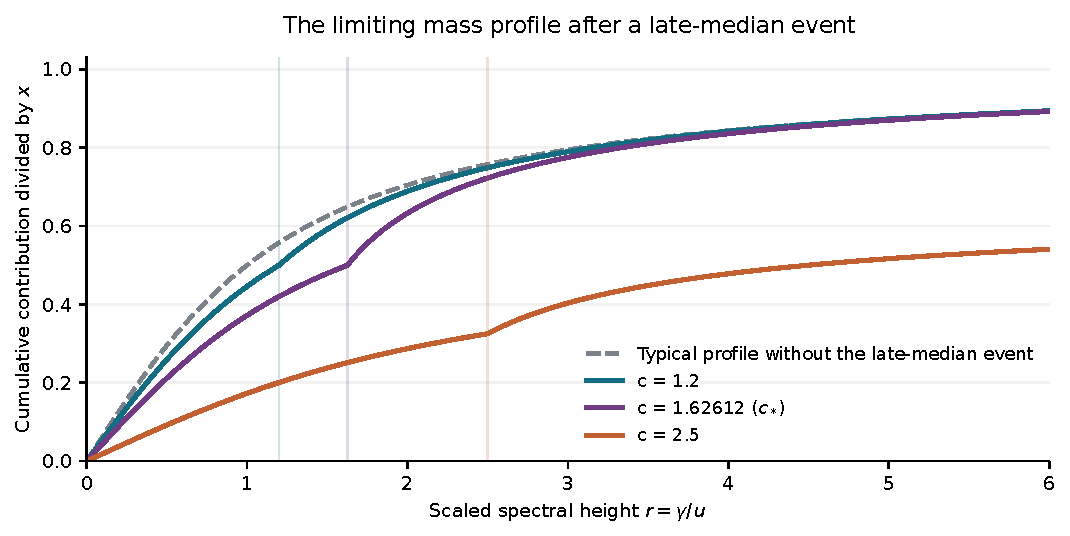
\includegraphics[width=0.94\textwidth]{figures/conditional_profiles.pdf}
 \caption{The cumulative limiting profiles in \cref{thm:profile} for the median, $\alpha=1$, $p=2$. Each colored curve conditions on a different late-median cutoff. The total of the $c=2.5$ curve, as $r\to\infty$, is $c_*/2.5=0.650448505958843\ldots$; its normalization is by $x$, not by its smaller realized total.}
 \label{fig:profiles}
\end{figure}

\section{Proof of the curvature jump}\label{sec:curvatureproof}

Near the transition, the integrals and their inverse parameters are smooth, because $a_*>0$ and $b_*>-c_*^p$. Thus $h(c,s)$ from \cref{eq:h} is smooth there. Below the transition the optimum is $h(c,C)$; above it the optimum is $h(c,s_0(c))$, where
\[
 s_0(c)=C(c_*/c)^{p-\alpha},\qquad
 s_0'(c_*)=-\frac{(p-\alpha)C}{c_*}.
\]
At $c_*$, $h_s=0$, so the first derivatives agree. Differentiating $h_s(c,s_0(c))=0$ yields
\[
 h_{cs}=-h_{ss}s_0'.
\]
The second derivative of the optimized value is
\[
 h_{cc}-\frac{h_{cs}^2}{h_{ss}},
\]
whereas the second derivative of the boundary value is $h_{cc}$. Their difference at $c_*$ is
\[
 h_{ss}\,s_0'(c_*)^2
 =\frac{(p-\alpha)^2C^2}{c_*^2}
 \left(\frac{\tau^2}{U}+\frac{(1-\tau)^2}{V}\right),
\]
which is strictly positive. This proves \cref{thm:curvature}. It is a genuine discontinuity of the second derivative, rather than merely a change between two representations of a smooth function.

\section{Explicit formulas for zeta-type spectra}\label{sec:explicit}

Take $\alpha=1$ and $p=2$. Then $C=D=\pi/2$ and
\begin{equation}\label{eq:Lexplicit}
 L_c(a)=\frac1{\sqrt a}\arctan\frac c{\sqrt a},
\end{equation}
while
\begin{equation}\label{eq:Rexplicit}
 R_c(b)=\begin{cases}
 b^{-1/2}\arctan(\sqrt b/c),&b>0,\\[0.2em]
 1/c,&b=0,\\[0.2em]
 (-b)^{-1/2}\arctanh(\sqrt{-b}/c),&-c^2<b<0.
 \end{cases}
\end{equation}
This expression is smooth through zero; for example
\[
 R_c(b)=c^{-1}-\frac b{3c^3}+\frac{b^2}{5c^5}+O(b^3).
\]
The typical quantile is $c_0=\tan(\pi\tau/2)$.

\begin{corollary}[Explicit transition at every quantile]\label{cor:explicit}
Let $k=\tau/(1-\tau)$ and let $w\in(0,1)$ be the unique root
\begin{equation}\label{eq:wgeneral}
 \arctan(\sqrt k/w)=\sqrt k\,\arctanh w.
\end{equation}
Then
\begin{equation}\label{eq:explicit_constants}
 A=\frac{w^2}{k},\qquad B=-w^2,\qquad
 c_* =\frac{2\arctanh w}{\pi(1-\tau)w},\qquad
 K=\log\frac{1+w^2/k}{1-w^2}.
\end{equation}
In the interior phase $\rate(c)=cK-\pi/2$ and $X/x\to c_*/c$. In the boundary phase, solve
\[
 L_c(a)=\tau\pi/2,\qquad R_c(b)=(1-\tau)\pi/2,
\]
and use
\begin{equation}\label{eq:explicit_boundary}
 \rate(c)=c\log\frac{c^2+a}{c^2+b}
 +\frac\pi2\{\tau a+(1-\tau)b-1\}.
\end{equation}
\end{corollary}

\begin{proof}
Substitute $B=-kA$ into \cref{eq:AB} and write $B=-w^2$, $A=w^2/k$. The explicit integrals in \cref{eq:Lexplicit,eq:Rexplicit} reduce the ratio equation to \cref{eq:wgeneral}. Its left side decreases in $w$ and its right side increases, with opposite endpoint orderings, proving existence and uniqueness. The remaining formulas follow from \cref{eq:cstar}.
\end{proof}

For the median, $\tau=1/2$, this gives \cref{eq:wmedian,eq:medianconstants} and proves \cref{thm:medianintro}. Numerically,
\[
 w=0.734095513758913\ldots,\qquad
 \mrate(c_*)=0.389001071095204\ldots.
\]
Selected values are shown in \cref{tab:rates}; the speed multiplying the rate is $\theta N(u)$.

\begin{table}[ht]
 \centering
 \caption{Median rates and total-mass limits. Values are numerical evaluations of exact formulas.}
 \label{tab:rates}
 \begin{tabular}{@{}rrr@{}}
 \toprule
 Cutoff $c$ & Rate $\mrate(c)$ & Limiting $X/x$ under both events \\
 \midrule
 1.05 & 0.002656117156 & 1 \\
 1.20 & 0.041625622399 & 1 \\
 1.40 & 0.162532536222 & 1 \\
 1.60 & 0.358125892904 & 1 \\
 $c_*$ & 0.389001071095 & 1 \\
 2.00 & 0.839598814325 & 0.813060632449 \\
 3.00 & 2.044796384885 & 0.542040421632 \\
 5.00 & 4.455191526006 & 0.325224252979 \\
 \bottomrule
 \end{tabular}
\end{table}

\subsection{A check against the earlier central limit theorem}

At the typical median cutoff $c=1$, the boundary rates are $a=b=1$. Direct differentiation gives
\begin{equation}\label{eq:curvature_typical}
 \mrate''(1)=\frac{4\pi}{\pi^2-4}
 =2.140922923532451\ldots,
 \qquad
 \mrate(c)=\frac{2\pi}{\pi^2-4}(c-1)^2+o((c-1)^2).
\end{equation}
Indeed, if
\[
 U_0=\int_0^1\frac{\dd r}{(1+r^2)^2}=\frac\pi8+\frac14,
 \qquad V_0=\frac\pi8-\frac14,
\]
then differentiating the boundary mean equations and \cref{eq:rate_derivative} gives
$\mrate''(1)=(U_0^{-1}+V_0^{-1})/4$, which is \cref{eq:curvature_typical}.

This agrees with the variance $(\pi^2-4)/(4\pi\theta N(u))$ obtained by translating the repository's median central limit theorem to scaled height. It checks the normalization of the large-deviation rate. It does \emph{not} justify replacing the exact or corrected center by one on the fluctuation scale: for Dirichlet zero counts, the repository proves that deterministic logarithmic corrections to that center dominate the Gaussian fluctuation scale. Our theorem keeps $c$ fixed beyond the typical cutoff and asserts no critical-window law.

\section{Arithmetic interpretation under the stated zero hypothesis}\label{sec:arithmetic}

The probabilistic result applies to any deterministic spectrum satisfying \cref{eq:RV}. The following specialization identifies the law from the source's completed-$L$-function construction.

\begin{corollary}[Reciprocal completed functions]\label{cor:arithmetic}
Take a fixed finite collection of copies of the Riemann $\xi$ function and completed nonprincipal primitive \emph{real} Dirichlet $L$-functions, with total number of degree-one factors $d\ge1$. Remove the central zero factor from each completed function. Assume RH and the corresponding Dirichlet GRH statements. Let $\gamma_j$ list all positive noncentral zero ordinates of these factors, with multiplicity, and let $\mathcal H(w)$ be their even product in the coordinate $s=1/2+w$ after removing those central factors. Then
\begin{equation}\label{eq:reciprocal}
 \frac{\mathcal H(w)}{\mathcal H(0)}
 =\prod_j\left(1+\frac{w^2}{\gamma_j^2}\right),
 \qquad
 \EE e^{-tX}=\left(\frac{\mathcal H(0)}{\mathcal H(\sqrt t)}\right)^\theta.
\end{equation}
All preceding results apply with $\alpha=1$, $p=2$. Moreover
\begin{equation}\label{eq:arith_scales}
 N(T)\sim\frac d{2\pi}T\log T,
 \qquad x\sim\frac{\theta d\log u}{4u},
\end{equation}
and, for every fixed $\tau\in(0,1)$ and $c>\tan(\pi\tau/2)$,
\begin{equation}\label{eq:arith_x_rate}
 \boxed{\lim_{x\downarrow0}\frac{x}{\log^2(1/x)}
 \log\PP(H_\tau>cu\mid X\le x)
 =-\frac{\theta^2d^2}{8\pi}\rate(c).}
\end{equation}
Here $u$ always denotes the exact saddle from \cref{eq:exact_saddle}.
\end{corollary}

\begin{proof}
Under the stated critical-line hypothesis, the paired Hadamard products of the completed functions, with their central factors removed, give \cref{eq:reciprocal}. Real characters have symmetric positive and negative ordinates; the functional equation and central-factor removal make the normalized product even. The reciprocal gamma-product law follows by multiplying the Laplace transforms of the independent gamma variables. This is the same factorization used in the source's small-deviation and conditioning results \cite{ProveIt,RoynetteYor,Gao}.

Summing the standard zero counts gives the first relation in \cref{eq:arith_scales}. The limit in \cref{eq:mu_limit}, with $C=\pi/2$, gives the second. Thus
\[
 u\sim\frac{\theta d}{4x}\log(1/x),\qquad
 \theta N(u)\sim\frac{\theta^2d^2}{8\pi x}\log^2(1/x).
\]
Substitute this speed into \cref{eq:rate_limit} to obtain \cref{eq:arith_x_rate}.
\end{proof}

\begin{remark}[Complex characters and precise scope]
The same identification extends to a fixed conjugation-closed multiset of nonprincipal primitive characters, with matching multiplicities for conjugate characters and all central factors removed. Pairing a nonreal character with its conjugate supplies an even product and counts as two degree-one factors. Without that closure, the probability theorem still applies to the chosen positive-ordinate spectrum, but one must not identify its paired product with the original unpaired completed functions. No uniformity in a growing conductor, degree, or family is asserted.
\end{remark}

\section{Reproducible checks and limits of the conclusion}\label{sec:verification}

The accompanying \texttt{code/verify.py} uses 70-decimal-digit arithmetic for constants and analytic cross-checks. It writes \texttt{data/verification.json}, \texttt{data/verification.txt}, and the vector figures included here. The following checks were executed successfully:
\begin{enumerate}
 \item The closed $L_c,R_c$ integrals were compared with independent quadrature at several quantiles and in both phases.
 \item The integration identity \cref{eq:IBP} was checked at independent arbitrary rates for four choices of $(\alpha,p)$, including nonintegral $\alpha$ and $p\ne2$.
 \item The rate, slope, and curvature calculations were matched at the transition; the curvature was also computed by implicit differentiation of the two boundary mean equations.
 \item Equation \cref{eq:curvature_typical} was checked independently against the earlier Gaussian variance.
 \item For the synthetic spectrum $\gamma_j=j$, exact gamma-product and digamma formulas were used to compute the discrete saddle at $u=25,50,100,200$ and compare it with the limiting saddle. No Monte Carlo approximation was used.
\end{enumerate}

For the last check, with $J=\lfloor cu\rfloor$ and $m=J+1$, the formulas include
\[
 \sum_{j\ge1}\frac1{j^2+z^2}
 =\frac{\pi z\coth(\pi z)-1}{2z^2},\qquad
 \prod_{j=m}^\infty\left(1+\frac{z^2}{j^2}\right)
 =\frac{\Gamma(m)^2}{\Gamma(m+iz)\Gamma(m-iz)}.
\]
The tail sum follows by differentiating the logarithm or using digamma differences. The domain is chosen so that every upper-band factor remains positive, including the negative-$b$ case. For instance, at $c=2$, the exact normalized discrete saddle rates for $u=25,50,100,200$ are approximately $0.8281731$, $0.8339282$, $0.8367740$, and $0.8381890$, approaching the limiting value $0.8395988$. These are exact-product \emph{saddle calculations}; they are not presented as exact finite-$u$ probabilities.

The numerical checks are independent consistency checks, not a substitute for the analytic proof or a certified interval computation. The exact equations define the theorem's constants. The new theorem has not been checked in Lean.

The limits hold for fixed $\tau\in(0,1)$ and fixed $c>c_0$. They do not establish uniform estimates as $\tau$ approaches an endpoint, as $c$ grows with $x^{-1}$, or as an arithmetic conductor grows. At $c=c_0$ the exponential rate is zero, and the limiting probability requires more precise centering. At $c=c_*$ the total still tends to $x$; a critical-window distribution for its smaller-scale slack is not proved here. All randomness is in the gamma weights on a deterministic spectrum, so the result makes no assertion that zeros themselves are random or independent.

\begin{thebibliography}{99}
\bibitem{ProveIt}
V. Reshetnikov, \emph{ProveIt: Analysis/GeneralizedRiemannHypothesis}, repository snapshot \commit, 27 November 2026. In particular \texttt{Article/sections/ana.tex} and the directory README.\\
\href{https://github.com/VladimirReshetnikov/ProveIt/tree/2e714ce3d8e33aa8160391cf5dd95f3af3c34045/Analysis/GeneralizedRiemannHypothesis}{Pinned repository snapshot and article sources}.

\bibitem{Sutherland}
A. V. Sutherland, \emph{Verification files for the shorter Lean proof of RH and of GRH for Dirichlet L-functions}, verification page, updated 27 November 2026, 17:27 UTC; accessed 27 November 2026.\\
\url{https://math.mit.edu/~drew/shortgrh/}

\bibitem{Saulis}
L. Saulis, \emph{Large deviation theorems for weighted summation of Gamma-distribution random variables}, Lietuvos matematikos rinkinys \textbf{42} (2002), 714--718. DOI: \href{https://doi.org/10.15388/LMR.2002.33064}{10.15388/LMR.2002.33064}.

\bibitem{Gozlan}
N. Gozlan, \emph{Conditional principles for random weighted measures}, ESAIM: Probability and Statistics \textbf{9} (2005), 283--306. DOI: \href{https://doi.org/10.1051/ps:2005016}{10.1051/ps:2005016}.

\bibitem{Gao}
F. Gao, J. Hannig, T.-Y. Lee, and F. Torcaso, \emph{Laplace transforms via Hadamard factorization}, Electronic Journal of Probability \textbf{8} (2003), paper 13.

\bibitem{RoynetteYor}
B. Roynette and M. Yor, \emph{Couples de Wald ind\'efiniment divisibles. Exemples li\'es \`a la fonction gamma d'Euler et \`a la fonction zeta de Riemann}, Annales de l'Institut Fourier \textbf{55} (2005), 1219--1283. DOI: \href{https://doi.org/10.5802/aif.2125}{10.5802/aif.2125}.

\bibitem{Sra}
S. Sra, \emph{On some positivity properties of the Riemann $\Xi$ function}, preprint, version 3, 2 November 2026, Appendix C.17; cited by the source repository.\\
\url{https://suvrit.github.io/papers/riem-xi/riem-xi-v3.pdf}

\bibitem{VanCampenhoutCover}
J. M. Van Campenhout and T. M. Cover, \emph{Maximum entropy and conditional probability}, IEEE Transactions on Information Theory \textbf{27} (1981), no.~4, 483--489.

\bibitem{MayerWolfZeitouni}
E. Mayer-Wolf and O. Zeitouni, \emph{The probability of small Gaussian ellipsoids and associated conditional moments}, Annals of Probability \textbf{21} (1993), no.~1, 14--24.
\end{thebibliography}
\end{document}
